\documentclass[a4paper,12pt]{article}
\usepackage[russian]{babel}   
\usepackage[utf8]{inputenc}  
\usepackage{xypic}
\usepackage{amssymb}
\usepackage{amsmath}
\usepackage{enumerate}
\usepackage{titlesec}
\usepackage[left=30mm, top=20mm, right=20mm, bottom=17.5mm, nohead, footskip=10mm]{geometry} % настройки полей документа
\usepackage{indentfirst}
\usepackage{setspace}
\usepackage{graphicx}
\graphicspath{{pics/}}
\DeclareGraphicsExtensions{.png}

\singlespacing

\begin{document}
    \section{Введение}
        Дадим некоторые базовые определения.
        Абелевой группой будем называть множество $G$ с определенной на нем операцией $+$ для которого выплонены следующие аксиомы:
        \begin{enumerate}
            \item $\forall a, b \in G$ $a + b \in G$
            \item $\exists 0 : a + 0 = 0 + a \in G$
            \item $\forall a \in G$ $\exists -a \in G : a + (-a) = 0$
            \item $\forall a, b \in G$ $a + b = b + a$
            \item $\forall a, b, c \in G$ $a + (b + c) = (a + b) + c$
        \end{enumerate}
        Проще говоря группой назовем множество элементы которого можно складывать, 
        вычитать и в котором имеется нейтральный элемент относительно данной операции.

        Сформулируем теорему Лагрнжа: пусть $H \subset G$ -- подгруппа в $G$, $n$ -- число элементов в $G$, $m$ -- число элементов в $H$. тогда
        $m | n$. Так же отметим важное свойство: для любого элемента $g \in G$ выполнено $ng = 0$.

        Предположим что мы сейчас работаем в $\mathbb{R}^2$.
        Дадим общее определение того что такое эллиптическая кривая. \textit{Эллиптической кривой} назовем множество точек $(x, y)$,
        удовлетворяющих уравнению $y^2 + a_1xy+a_3y = x^3+a_2x^2+a_4x + a_5$, где $a_i$ -- некоторый числа.
        Множество таких точек обозначим как 
        $$
            E = \{(x, y) | y^2 + a_1xy+a_3y = x^3+a_2x^2+a_4x + a_5\}.
        $$

        Это было достаточно общее определение, далее будем предполагать что эллиптическая кривая задана уравнением
        $y^2 = x^3 + ax + b$. Далее картинка на которой показана зависимость множества точек от параметров $a, b$.

        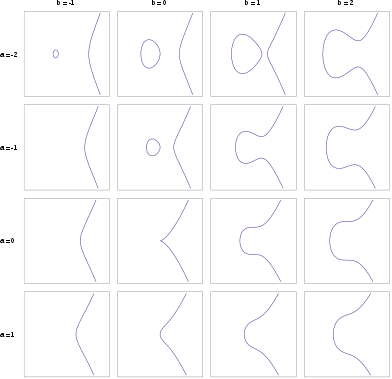
\includegraphics{EC}

        Как можно видеть, имеем 2 разные ситуации: когда график кривой представляет из себя множество, состоящие из одной связной 
        компоненты и из двух. Так же можно видеть, что при некоторый значениях параметров возникают особенности: кривая может пересечь саму себя,
        а так же есть точка излома. Кривые, обладающие такими особенностиями называют вырожденными. Для определения всех этих ситуаций введем
        понятие \textit{дискриминанта}. \textit{Дискриминантом} эллиптической кривой назовем величину 
        $$
            \Delta = -16(4a^3 + 27b^2)
        $$ 
        Если $\Delta < 0$, то кривая имеет две компоненты, если $\Delta > 0$, то кривая имеет одну компоненту. Если же
        $\Delta = 0$, то кривая является вырожденной.

        Далее будем предполагать что кривая является невырожденной, то есть ее дискриминант отличен от нуля. 

        Последнее что нам потребуется это ввести понятие бесконечно удаленной точки. Чтобы не углубляться в науку скажем что это точка, находящаяся где-то
        за пределами плоскости и принадлежащая нашей эллиптической кривой. Таким образом будем рассматривать кривые вида
        $$
            E = \{(x, y) | y^2 = x^3 + ax + b, -16(4a^3 + 27b^2) \neq 0\} \cup \{\infty\}
        $$

    \section{Сложение точек на кривой}
        Введем понятие нейтрального элемента. Нейтральным элементом относительно нашего сложения назовем бесконечно удаленную точку.

        Определим сумму трех точек эллиптической кривой. Сумма трех точек $P, Q, R'$ равна нулю, если эти три точки лежат
        на одной прямой. 

        Введем понятие обратного элемента. Противоположной к точке $P = (x_P, y_P)$ является точка $-P = (x_P, -y_P)$. Проверим что это так.
        Действительно, в качестве третий точки возьмем $\infty$, и проведем прямую, получим что $P + (-P) + 0 = 0$. 

        Из такого геометрического определения видно, что операция коммутативна и ассоциативна. 

        Теперь научимся по заданным координатам точек и уравнению кривой вычислять их сумму. Пусть заданы две точки $P = (x_P, y_P)$ и
        $Q = (x_Q, y_Q)$. Вычислим точку $R$, которая удовлетворяет соотношению $P + Q + R = 0$. Предположим, что $Q \neq -P$ и $Q \neq 0$,
        так как в этих случаях ответ очевиден. Раз точки не лежат на вертикальной прямой, то мы можем определить коэффициент наклона $k$ прямой,
        проходящей через эти точки. Теперь подставим уравнение полученной прямой в уравнение эллиптической кривой и получим что
        $$
            x_R = k^2 - x_P - x_Q,\;
            y_R = y_P + k(x_R - x_P)
        $$
        В случае $P = Q$ проводим касательную, для которой $k = \mp\frac{3x_P^2 + a}{2y_P}$. Это ничто иное, как коэффициент нахклона
        касательной к графику функции $y = \pm\sqrt{x^3 + ax + b}$.

        Примеры: $y^2 = x^3 - 7x + 10$, $P = (1, 2)$, $Q = (3, 4)$, $P = Q = (1, 2)$.

        Теперь введем понятие умножения точки на целое число. Пусть задано $n \in \mathbb{Z}$, $n~>~0$, тогда $nP = \underbrace{P + P + \dots + P}_{n\;\text{раз}}$. 
        Если же $n < 0$, то $nP = \underbrace{(-P) + (-P) + \dots + (-P)}_{-n \; \text{раз}}$

        Здесь можно отметить следующий факт: чтобы вычислить $nP$ потребуется порядка $\log_2{n}$ операций, что достаточно быстро, в
        то время как по $nP$ и $P$ найти $n$ достаточно сложно. Эта задача называется проблемой дискретного логарифмирования.

    \section{Эллиптические кривые над кончеными полями}
        Теперь рассмотрим случай, когда основным полем является не $\mathbb{R}$, а $\mathbb{Z}_p$, где $p$ -- простое 
        число большее 3. Опредление эллиптической кривой над $\mathbb{Z}_p$ никак не меняется. Это так же множество точек, которые удовлетворяют
        заданному уравнению. Все что измениться -- формулы сложения точек. В формулах для случая на $\mathbb{R}$ достаточно заменить деление взятием обраного по
        модулю $p$. Обратный элемент можно найти с помощью расширенного алгоритма Евклида. 
        
        В данной ситуации возникает вопрос о количестве точек эллиптической кривой. На нейго отвечает теорема Хассе, утверждающая, что число точек на эллиптической кривой над 
        $\mathbb{Z}_p$ близко к числу $p$.

    \section{Циклическая группа точки кривой}
        Важным для дальнейшего понимания алгоритмов криптографии на эллиптических кривых явялется понятие циклической группы. Обозначим через $N$ -- количество точек на кривой.
        Заметим, что для любой точки $P$ верно равенство $N \cdot P = 0$.
        Рассмотрим некоторую точку $P$ на кривой над $\mathbb{Z}_p$ и будем ее 
        последовательно умножать на числа $1, 2, \dots, n, \dots$ до тех пор пока результат не станет равен нулю. 
        Полученное множество точек $\{0, P, 2P, \dots, (n-1)P\}$ будем называть  циклической группой, порожденной точкой $P$. 
        Число $n$ назывется порядком группы, а число $h = N / n$ -- кофактор группы. Утверждается что число $h$ всегда целое. Теперь можно
        вывести одно очень важное равенство: $n(hP) = 0$. 
\end{document}